\documentclass[a4paper, 12pt]{article}
\setcounter{secnumdepth}{3}
\setcounter{tocdepth}{2}

%% Språk och font
\usepackage[swedish]{babel}
%\usepackage[utf8x]{inputenc}
\usepackage[T1]{fontenc}
\usepackage[utf8]{inputenc}
\usepackage{biblatex}
\usepackage{dirtytalk}

%% Sätter pappersstorlek och marginaler
\usepackage[a4paper,top=2.5cm,bottom=2.5cm,left=2.5cm,right=2.5cm,marginparwidth=1.75cm]{geometry}

%% Gör att figurer namnges efter kapitel
\usepackage{chngcntr}
\counterwithin{figure}{section}

%% Användbara paket
\usepackage{amsmath}
\usepackage{amssymb}
\usepackage{graphicx}
\usepackage{subcaption}
\usepackage{caption}
\usepackage{float}
\usepackage[colorinlistoftodos]{todonotes}
\usepackage[colorlinks=true, allcolors=black]{hyperref}
\usepackage{enumerate}
\usepackage{amsthm}
\usepackage{textcomp}
\usepackage{gensymb}
\usepackage{csquotes}
\let\micro\micro
\let\perthousand\perthousand
\usepackage{listings}
\lstset{
  basicstyle=\ttfamily,
  columns=fullflexible,
  frame=single,
  breaklines=true,
  postbreak=\mbox{\textcolor{red}{$\hookrightarrow$}\space},
}

%% Sats-environment
\theoremstyle{definition}
\newtheorem{exmp}{Exempel}[section]
\newtheorem*{lsn}{Lösning}
\newtheorem{sats}{Sats}[section]
\newtheorem{definition}{Definition}[section]
\newtheorem*{anm}{Anmärkning}
\newtheorem{uppg}{}[subsection]

%% Figurer
\usepackage{siunitx}
\setlength{\parindent}{0pt}
\setlength{\parskip}{10pt}
\setlength{\fboxsep}{.5\fboxsep}
\newcommand{\mrel}{\mathrel{\bigcirc}}

%% För tabeller
\usepackage{array}
\usepackage{tabularx}
\newcolumntype{L}[1]{>{\raggedright\let\newline\\\arraybackslash\hspace{0pt}}m{#1}}
\newcolumntype{C}[1]{>{\centering\let\newline\\\arraybackslash\hspace{0pt}}m{#1}}
\newcolumntype{R}[1]{>{\raggedleft\let\newline\\\arraybackslash\hspace{0pt}}m{#1}}

%% Titel och författare
\title{Corona virus modell}
\author{}
\date{Data till och med 17 april 2020 används i resultat} %För inget datum

%\linespread{1.25}, for increased spacing

\begin{document}
\maketitle
\section{Introduktion}
I denna rapport presenteras en modell som har använts och anpassats för att prediktera antalet fall av Coronaviruset Covid-19. Syftet med denna prediktion är att ha en skattning för hur många sjukvårdsplatser som behövs för inlagda patienter som mest under sjukdomsförloppet samt att undersöka när detta kommer att ske.

Det skulle gå att prediktera antalet personer med hjälp av statistisk regression eller liknande där man sätter upp en statistisk modell. Detta skulle kunna vara exempelvis exponentiell eller linjär tillväxt. Nackdelen med dessa två modeller är att antalet sjuka patienter just nu går mot oändligheten, vilket inte är rimligt långsiktigt eftersom personer bli immuna.

Modellen som används i denna rapport har tagit sin inspiration från Lotka-Volterras ekvationer, vilka beskriver hur många individer det finns av två arter (som kallas byten och rovdjur) över tid. Denna utgår från att antalet rovdjur ökar då antalet byten är stort och vice versa. Se \url{https://en.wikipedia.org/wiki/Lotka%E2%80%93Volterra_equations}.

\section{Modellen}
\subsection{Modellens uppbyggnad}
I modellen säger vi att det finns fem olika kategorier av individer vid varje given tidpunkt. Dessa kategorier är beskrivna i följande tabell:

\begin{center}
  \begin{tabular}{p{3cm} | p{8cm}}
    \textbf{Kategori} & \textbf{Beskrivning} \\ \hline
    Risk & De som riskerar bli sjuka, alltså ej haft sjukdomen än \\ \hline
    Sjuka & De som just nu har sjukdomen \\ \hline
    Inlagda & De som just nu har sjukdomen och uppsöker vård, detta är en delmängd av alla sjuka \\ \hline
    Immuna & De som har haft sjukdomen och nu är immuna \\ \hline
    Döda & De som avlidit med sjukdomen
  \end{tabular}
\end{center}

Enligt vår modell färdas individer genom följande:
\begin{figure}[H]
\centering
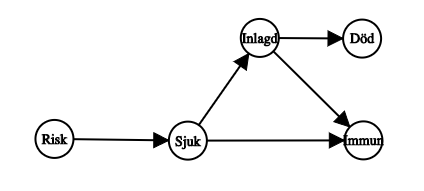
\includegraphics[width=0.6\textwidth]{bilder/flow.png}
\caption{Figur som visar hur en individ färdas mellan de olika kategorierna.}\label{Fig: flow}
\end{figure}
Som vi ser färdas individerna endast enligt pilarnas riktning och går aldrig tillbaka. I vår modell antar vi också att ''Inlagda'' är en delmängd av alla sjuka. Vi antar i modelleringen att alla individer finns i exakt en av grupperna ''Risk'', ''Sjuka'', ''Immuna'' och ''Döda''.

\subsection{Beskrivning av flödet mellan kategorierna}
Vi börjar med att införa beteckningar för hur många individer det finns i varje kategori. För att göra detta låter vi:
\begin{align*}
  r(t) &= \text{Antal i Risk vid tiden t} \\
  s(t) &= \text{Antal Sjuka vid tiden t} \\
  a(t) &= \text{Antal Inladga vid tiden t} \\
  i(t) &= \text{Antal Immuna vid tiden t} \\
  d(t) &= \text{Antal Döda vid tiden t}
\end{align*}
Vi mäter tiden $t$ i dagar. Notera att $r(t)+s(t)+i(t)+d(t)$ antas vara konstant för alla $t$, eftersom vi antar att alla individer befinner sig i exakt en av dessa fyra grupper. Anledningen till att just $r(t)+s(t)+i(t)+d(t)$ är konstant och inte $r(t)+s(t)+i(t)+d(t)+a(t)$ är konstant är att en patient kan vara både i gruppen ''Sjuka'' och ''Inlagda'' samtidigt. Men om en patient är i gruppen ''Inlagda'' är den också i gruppen ''Sjuka''.

Vi går igenom varje pil för sig i figur \ref{Fig: flow} för att förklara antaganden.

Antalet personer som går från Risk till Sjuka antar vi är proportionellt mot antalet möten mellan sjuka och riskindivider. Det betyder att vi antar att antalet som går från Risk till Sjuka kan beskrivas som $\beta r(t)s(t)$, där $\beta$ är en positiv konstant. Detta kommer från att antalet möten mellan individer från Risk och Sjuka antas vara proportionellt mot $r(t)s(t)$.

Vidare antar vi att andelen som är Inlagda, alltså uppsöker sjukvård, är en lika stor andel av alla sjuka hela tiden. Låt denna andel kallas $\gamma$, alltså har vi $a(t)=\gamma s(t)$.

Vi antar att individer är sjuka under $L$ dagar vilket gör att $L$ dagar efter att en individ blir sjuk blir denna antingen immun eller död. Vi antar också att en sjuk individ smittar lika mycket under hela sjukdomsförloppet, samt att en sjuk individ är inlagd under hela sjukdomsförloppet eller inte alls. Dessa två antaganden är givetvis inte helt samstämmande med hur det faktiskt är, men är approximationer som används. Detta kan också ses som att en individ i gruppen ''Sjuka'' är när individen faktiskt är smittspridare.

Antag att andelen som dör är $\alpha$. Från detta ges hur förändringen av antal immuna och döda beror på hur många individer som gick från risk till sjuka var $L$ dagar tidigare.

Dessa beskrivningar kan sammanfattas med följande matematiska formler. Notera att för en funktion $f(t)$ beteckar $f^\prime(t)$ derivatan, alltså förändringen, av funktionen.

\begin{align}\label{Eq: Movement}
  i^\prime(t) &= (1-\alpha)\beta r(t-L)s(t-L) \\
  d^\prime(t) &= \alpha\beta r(t-L)s(t-L) \\
  s^\prime(t) &= \beta s(t)r(t) - \beta r(t-L)s(t-L) \\
  r^\prime(t) &= -\beta s(t)r(t)\\
  a(t) &= \gamma s(t)
\end{align}

För att underlätta beräkningar diskretiserar vi modellen och låter $f_x$ beteckna värdet av $f$ vid dag $x$, alltså $f(x)$. Skillnaden är att nu kan vi bara betrakta $f_x$ för heltal $x$, inte vilket värde som helst. Derivatan av en funktion $f^\prime(x)$ ersätter vi med $f_x-f_{x-1}$. Vi ändrar också lite grann i ekvationerna från \ref{Eq: Movement} för att hela tiden kunna skapa en skattning från en dag till nästa. Denna skillnad är att vi antar att antalet som går från Risk till Sjuka dag $t$ är proportionellt mot antalet möten mellan personer i Risk och Sjuka dag $t-1$, vilket inte förefaller orimligt. Det ger oss:

\begin{align}\label{Eq: Movement Diskret}
  i_t-i_{t-1} &= (1-\alpha)\beta r_{t-L}s_{t-L} \\
  d_t-d_{t-1} &= \alpha\beta r_{t-L}s_{t-L} \\
  s_t-s_{t-1} &= \beta s_{t-1}r_{t-1} - \beta r_{t-L}s_{t-L} \\
  r_t-r_{t-1} &= -\beta s_{t-1}r_{t-1}\\
  a_t &= \gamma s_t
\end{align}

Dessa antaganden och ekvationer ger ett sätt att givet hur många som finns i respektive kategori en dag förutspå dagen efter. Denna procedur kan sedan upprepas godtyckligt långt vilket ger att en fullständig tidsserie kan skapas. För att få en bra prediktion krävs dock att (förutom att antagandena inte är för långt ifrån verkligheten) att parametrarna $\alpha,\beta,\gamma,L$ väljs på ett korrekt sätt. Dessa bör väljas så att modellen som vi har är så nära den observerade datan som möjligt.

Den data vi har tillgängligt som observationer är för $a_t$ och $d_t$. Vi vill alltså välja parametrarna så att dessa värden stämmer överens med observationerna som finns. Det som återstår att förklara är hur parametrarna väljs, vilket beskrivs i kommande avsnitt.

\subsection{Val av parametrar}
För att hitta optimala parametrar försöker vi anpassa parametrarna så att $a_t$ och $d_t$ stämmer så väl överens med de observerade värdena som möjligt. Först testades ett antal parameterkonfigurationer manuellt för att hitta av vilken storleksordning alla parametrar ska vara. Då gavs det att parametrarna ska vara ungefär i följande intervall:
\begin{center}
  \begin{tabular}{c | c}
    \textbf{Parameter} & \textbf{Ungefärligt Värde} \\ \hline
    $\alpha$ & $[10^{-4},10^{-3}]$ \\ \hline
    $\beta$ & $[10^{-7},2\cdot 10^{-7}]$ \\ \hline
    $\gamma$ & $[10^{-3},2\cdot 10^{-3}]$ \\ \hline
    $L$ & $[4,14]$
  \end{tabular}
\end{center}
Notera att vi här inte angivit $K$, alltså antalet individer som var sjuka då vi startar testet. Anledningen till detta är att vi hela tiden kommer att använda ett $K$ sådant att $K\cdot \gamma=3$, eftersom det är ungefär 3 individer som är inlagda vid testets början.

Därefter låter vi programmet testa modeller med parametrar i dessa intervall och välja den ''bästa'' modellen. För att välja den bästa modellen måste vi definiera vad en ''bra'' modell är, och skapa en metrik för hur ''bra'' en modell är. Vi gör detta genom att skapa en ''felfunktion'' och därefter säga att den bästa modellen är den modell som minimerar felfunktionen. Vi återkommer i delavsnitt \ref{Subsub: felfunktioner} till vilka felfunktioner som har använts.

Det som programmet praktiskt sett gör är att ge varje parameter en lista av värden som den ska testa. Dessa listor är:
\begin{center}
  \begin{tabular}{c | c}
    \textbf{Parameter} & \textbf{Lista} \\ \hline
    $\alpha$ & $\{ 1\cdot10^{-4},2\cdot10^{-4},\ldots,10\cdot10^{-4}\}$ \\ \hline
    $\beta$ & $\{ 10\cdot10^{-8},11\cdot10^{-8},\ldots,19\cdot10^{-8} \}$ \\ \hline
    $\gamma$ & $\{ 8\cdot10^{-4},9\cdot10^{-4},\ldots,25\cdot10^{-4} \}$ \\ \hline
    $L$ & $\{ 4,5,\ldots,12 \}$
  \end{tabular}
\end{center}
Därefter använder programmet dessa parametrar för att simulera hur många individer det finns i varje grupp över tid. Därefter jämförs värdena för $a_t$ och $d_t$ med de observerade. Det betyder att vi testar totalt $10\cdot 10\cdot 18\cdot 9=16200$ olika modeller. För varje av dessa beräknar vi sedan hur fel skattning modellen ger genom att beräkna felfunktionen för varje modell. Den parameterkonfigurationen som ger det minsta felet säger vi sedan är den bästa modellen.

Notera här att vi söker parametrar som ger en så bra modell som möjligt. Det som programmet får fram är den bästa modellen av alla de vi testat. Förhoppningen då är att parametrarna som vi får är så nära som möjligt de faktiskt bästa parametrarna. En viktig sak då det är att om vi ser att en parameter i den modellen vi får är den bästa är det största eller minsta värdet vi testat på denna parameter så bör vi bli skeptiska. Anledningen till detta är att det mycket väl skulle kunna vara så att om vi gör parameterna ännu större respektive mindre så kommer modellen bli ännu bättre. Vi vill därför när vi fått fram de optimala parametrarna se till att parametervalen faktiskt inte är det största eller minsta. Notera att vi fortfarande inte vet om vi faktiskt är nära en optimal modell, men detta är ett sätt att troliggöra det mer i varje fall.

\subsubsection{Felfuktioner som använts}\label{Subsub: felfunktioner}
Två felfunktioner har använts. Båda dessa bygger på att vi vill minimera det genomsnittliga kvadratfelet mellan vår prediktion och det som observerats. Låt $a_t,d_t$ vara de värden vi predikterat för antalet inlagda och antalet döda vid tidpunkten $t$. Vidare, låt $a_t^{obs},d_t^{obs}$ vara de värden vi observerat för antalet inlagda och antalet döda vid tidpunkten $t$. Låt $T$ vara antalet dagar efter den första dagen som vi ska använda för att optimera parametrarna.

Den första felfunktionen är bara att vi tar det genomsnittliga kvadratfelet mellan observationerna och prediktionerna, samt att vi ger kvadratfelet för antalet inlagda vikten $w$ och för antalet döda vikten $1-w$. Detta ger att vår felfunktion, vi kallar felfunktioner $e(parametrar)$ eftersom de beror på parametrarna som valts, ges av:
\begin{equation}
  e_{GKF}(parametrar) = w\cdot \frac{1}{T+1}\sum_{t=0}^T (a_t-a_t^{obs})^2 + (1-w)\cdot \frac{1}{T+1}\sum_{t=0}^T (d_t-d_t^{obs})^2
\end{equation}
$GKF$ i $e_{GKF}$ står här för Genomsnittligt KvadratFel. Här kan $w$ väljas för att ge olika vikt åt antalet döda och antalet inlagda. I programmet används $w=0.8$ per default, eftersom båda värdena är viktiga att de överensstämmer med verkligheten, men vi önskar egentligen framför allt prediktera antalet inlagda, därför får dess kvadratfel större vikt.

Den andra felfunktionen som använts vill ta hänsyn till att det är viktigare att modellen predikterar bra närmre då den ska prediktera. En modell ska prediktera framtiden, alltså om vi är vid dag $T$ så vill vi prediktera dag $T+1$, $T+2$, osv. Det betyder att det skulle kunna vara önskvärt att ha en modell där dagarna precis innan, alltså dag $T, T-1, T-2$, osv är väldigt nära observationerna även om det gör så att dagarna längre tillbaka är längre ifrån kommer vara mer fel. Det gör att vi lägger till ytterligare en parameter, $w_e$, som är en exponentiell vikt, där $0<w_e\leq 1$. (Denna felfunktion är inspirerad av EWMA, alltså Exponentially Weighted Moving Average, se \url{https://en.wikipedia.org/wiki/Moving_average#Exponential_moving_average}.) Denna felfunktion ges då av:
\begin{equation}
  e_{EVGKF}(parametrar) = w\cdot \frac{1}{\sum_{t=0}^T w_e^{T-t}}\sum_{t=0}^T w_e^{T-t}(a_t-a_t^{obs})^2 + (1-w)\cdot \frac{1}{T+1}\sum_{t=0}^T w_e^{T-t}(d_t-d_t^{obs})^2
\end{equation}
$EVGKF$ i $e_{EVGKF}$ står här för Exponentiellt Viktat Genomsnittligt KvadratFel. Här kan $w$ väljas för att ge olika vikt åt antalet döda och antalet inlagda. I programmet används $w=0.8$ per default, eftersom båda värdena är viktiga att de överensstämmer med verkligheten, men vi önskar egentligen framför allt prediktera antalet inlagda, därför får dess kvadratfel större vikt. Här kan även $w_e$ väljas så att betydelsen av hur snabbt hur nära modellen är observationerna längre bak i tiden tappar betydelse. I programmet används $w_e=0.9$, vilket innebär att det är ungefär hälften så viktigt att modellen är nära observationerna för en vecka sedan som det är att att modellen är nära observationerna idag. Notera att om $w_e=1$ används så ges felfunktionen utan exponentiell viktning.

\section{Resultat}
Varje dag som Region Skåne publicerar ny data på  gällande antal inlagda och antal döda kan, och bör, programmet köras. Genom att använda all data till och med 17 april ges följande val av parametrar:
\iffalse \url{https://www.skane.se/digitala-rapporter/lagesbild-covid-19-i-skane/inledning/} \fi
\begin{center}
  \begin{tabular}{c | c | c}
    \textbf{Parameter} & \textbf{Värde felfunktion $e_{GKF}$} & \textbf{Värde felfunktion $e_{EVGKF}$} \\ \hline
    $\alpha$ & $0.0004$ & $0.0002$\\ \hline
    $\beta$ & $1.3\cdot 10^{-7}$ & $1.5\cdot 10^{-7}$ \\ \hline
    $\gamma$ & $0.0012$ & $0.0009$\\ \hline
    $K$ & 2500 & 3333 \\ \hline
    $L$ & 8 & 7
  \end{tabular}
\end{center}
Det ger följande prediktioner för parametrarna som ges med $e_{GKF}$:
\begin{figure}[H]
\centering
\begin{subfigure}[b]{.49\textwidth}
\centering
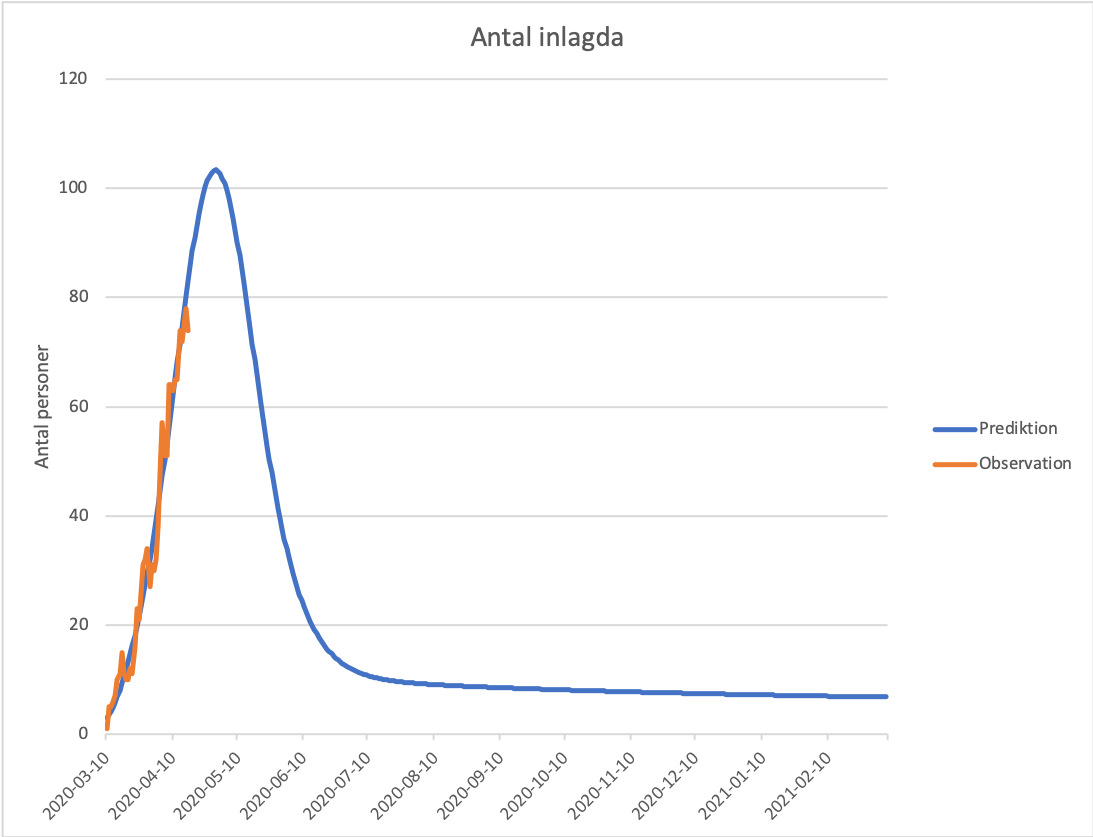
\includegraphics[width=.9\hsize]{bilder/antal_inlagda_predikterat_20200417_gkf.png}
\caption{Antal inlagda.}
\end{subfigure}
\begin{subfigure}[b]{.49\textwidth}
\centering
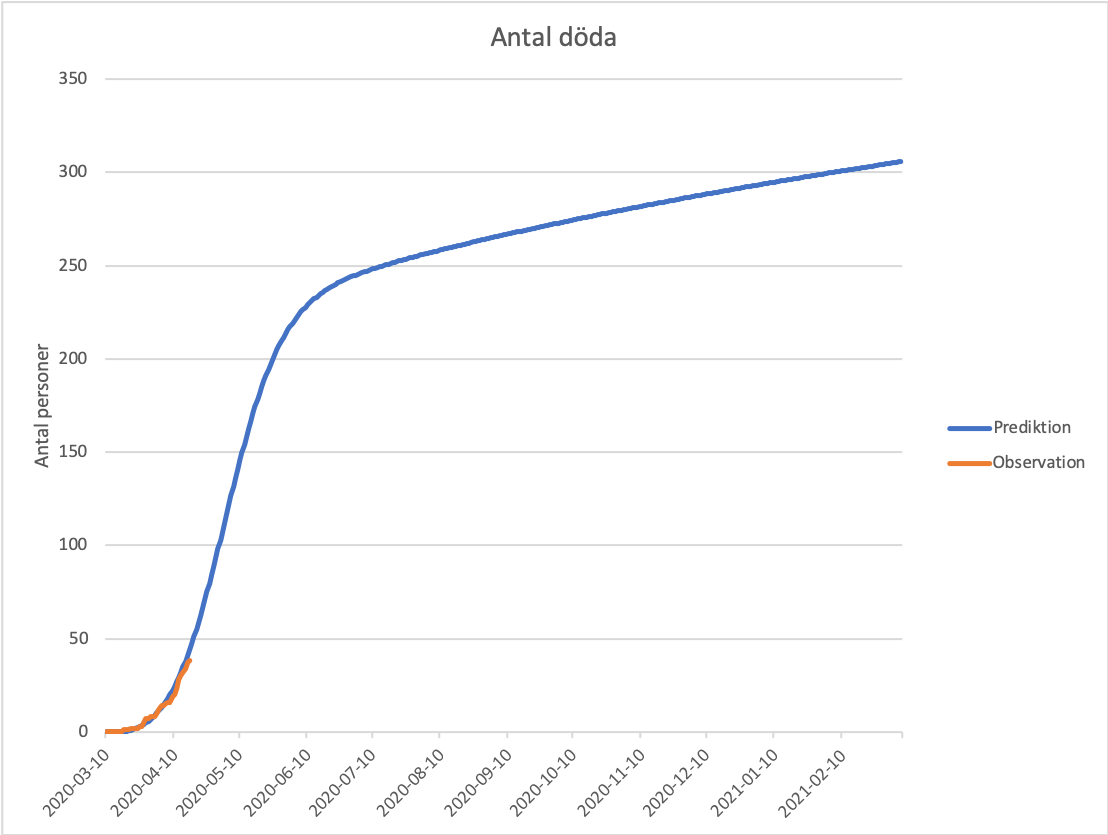
\includegraphics[width=.9\hsize]{bilder/antal_doda_predikterat_20200417_gkf.png}
\caption{Totalt antal döda}
\end{subfigure}
\caption{Prediktion med parametrar som ges av felfunktion $e_{GKF}$.}
\end{figure}

Prediktionerna med parametrarna som ges med $e_{EVGKF}$ är:
\begin{figure}[H]
\centering
\begin{subfigure}[b]{.49\textwidth}
\centering
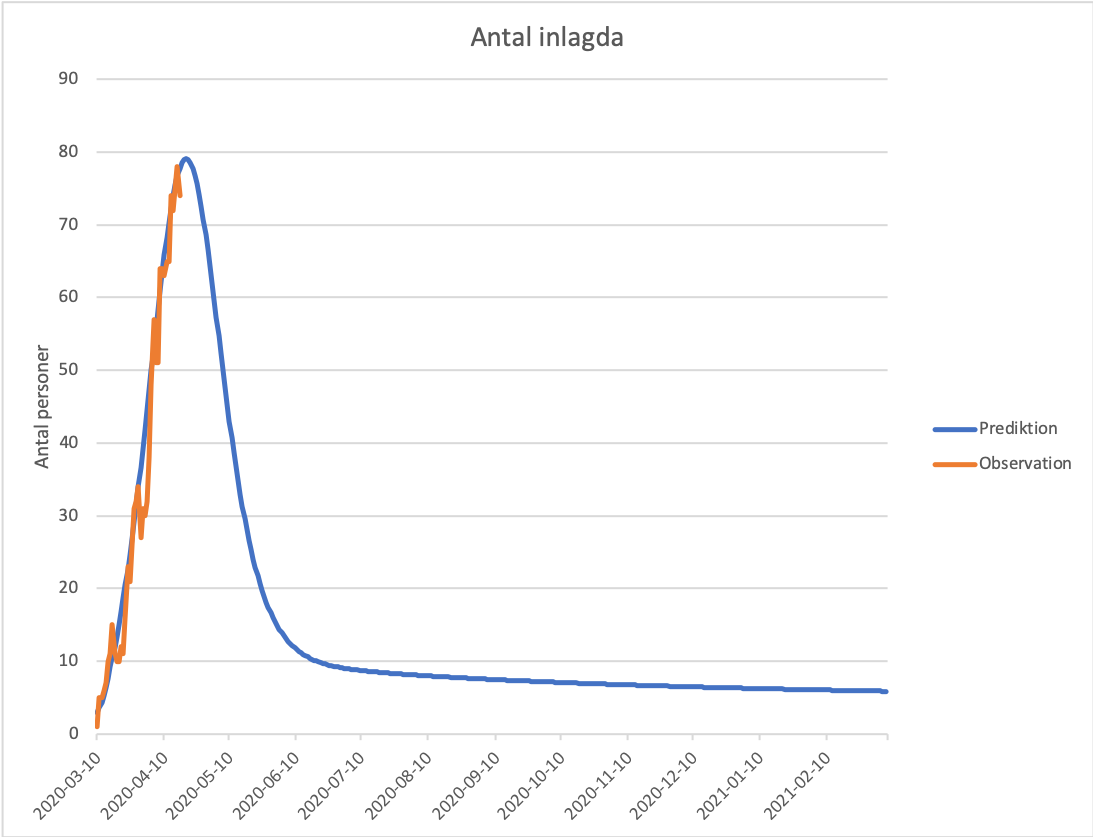
\includegraphics[width=.9\hsize]{bilder/antal_inlagda_predikterat_20200417_evgkf.png}
\caption{Antal inlagda}
\end{subfigure}
\begin{subfigure}[b]{.49\textwidth}
\centering
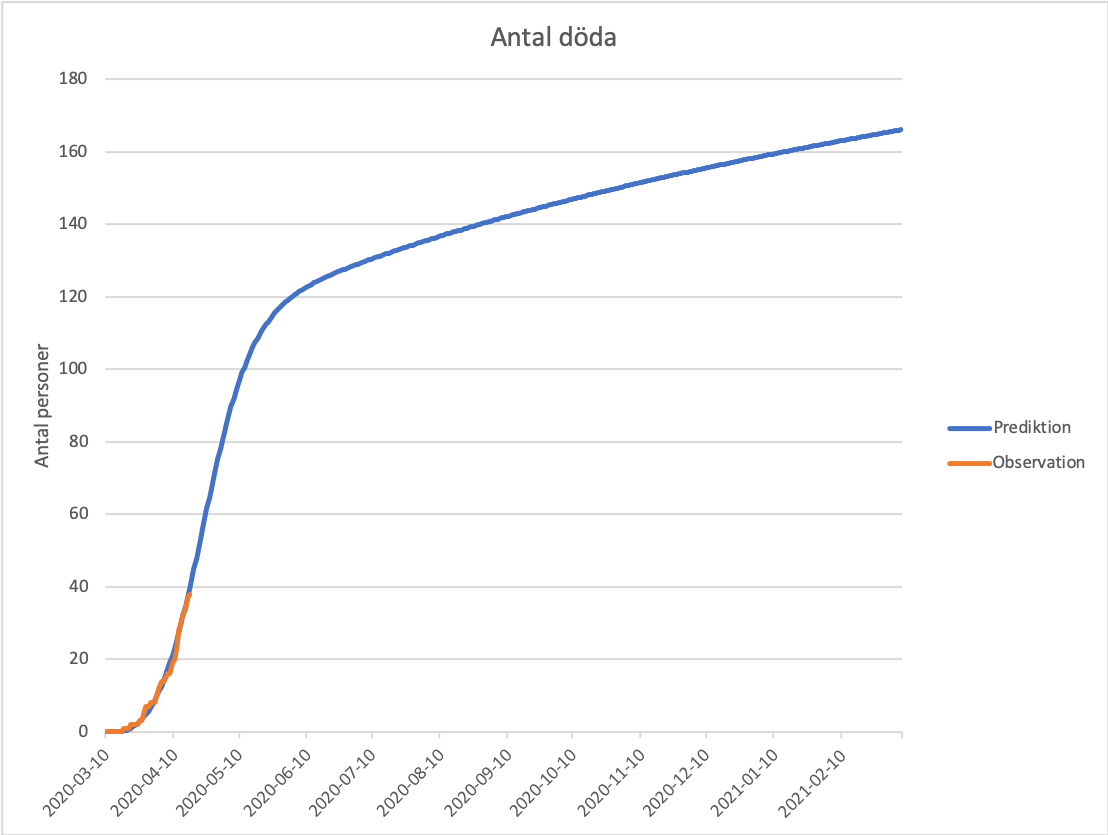
\includegraphics[width=.9\hsize]{bilder/antal_doda_predikterat_20200417_evgkf.png}
\caption{Totalt antal döda}
\end{subfigure}
\caption{Prediktion med parametrar som ges av felfunktion $e_{EVGKF}$.}
\end{figure}
Med hjälp av dessa modeller kan vi skatta tidpunkten och storleken på toppen av behovet av platser för inlagda individer. Dessa ges av:
\begin{center}
  \begin{tabular}{c | c | c}
     & \textbf{Dag för topp} & \textbf{Storlek på topp} \\ \hline
    \textbf{Modell med felfunktion $e_{GKF}$} & 2020-04-30 & 103 \\ \hline
    \textbf{Modell med felfunktion $e_{EVGKF}$} & 2020-04-20 & 79
  \end{tabular}
\end{center}

\subsection{Osäkerhet hos modellerna}
För att se hur osäker prediktionerna är, kan vi tänka oss följande. Om parametrarna inte ändras så mycket, så är prediktionerna snarlika. Därför kan vi betrakta hur parametrarna ändras över tiden. Därför skattar vi parametrarna som gavs om körningen gjordes för varje dag från dag 14 efter att vår observerade data börjar så långt som det går. Då får vi följande parametrar som är optimala:
\begin{figure}[H]
\centering
\begin{subfigure}[b]{.49\textwidth}
\centering
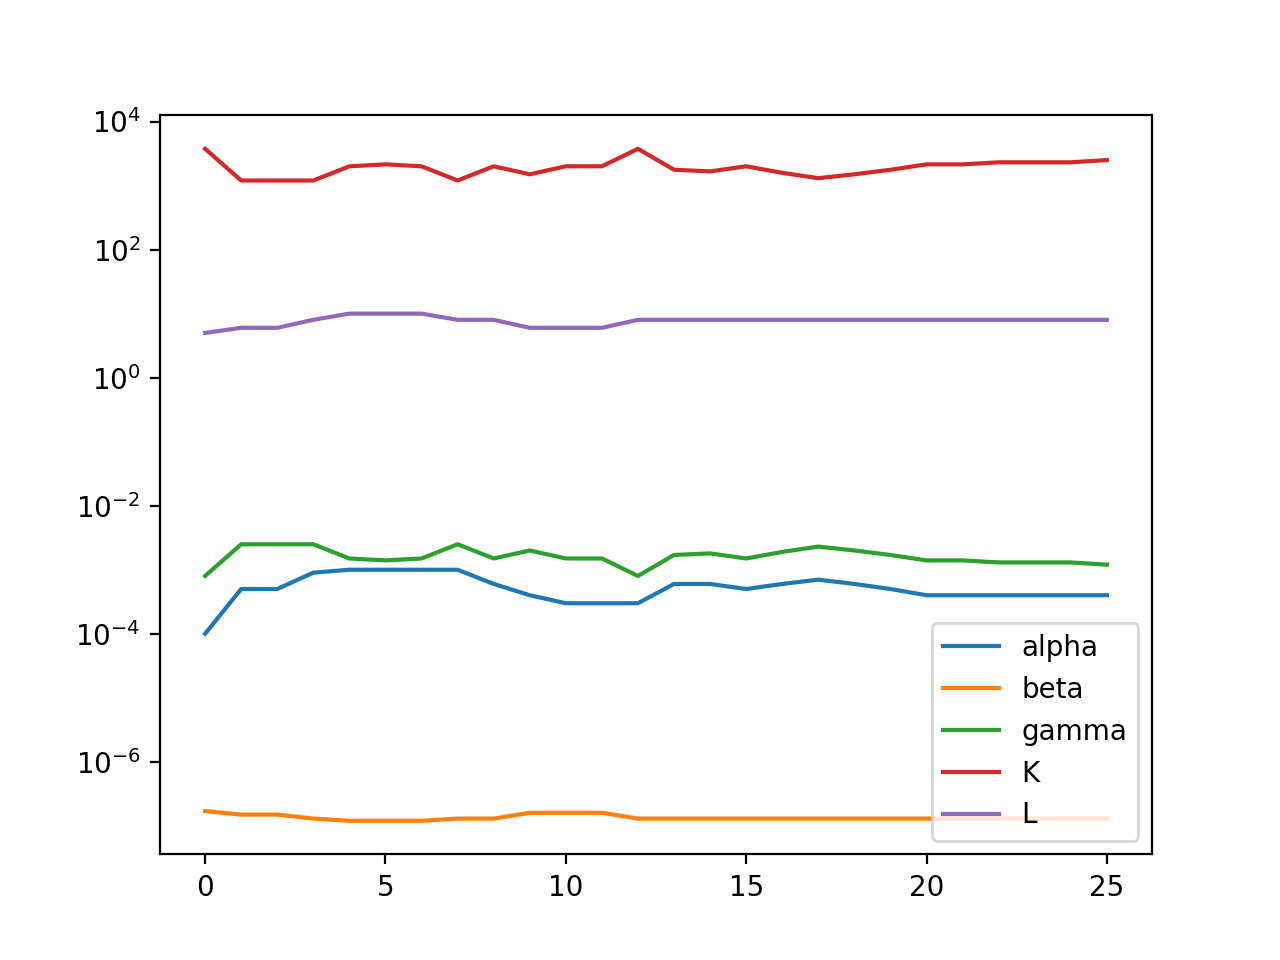
\includegraphics[width=.9\hsize]{bilder/parametrar_over_tid_20200417_gkf.png}
\caption{Med felfunktion $e_{GKF}$}
\end{subfigure}
\begin{subfigure}[b]{.49\textwidth}
\centering
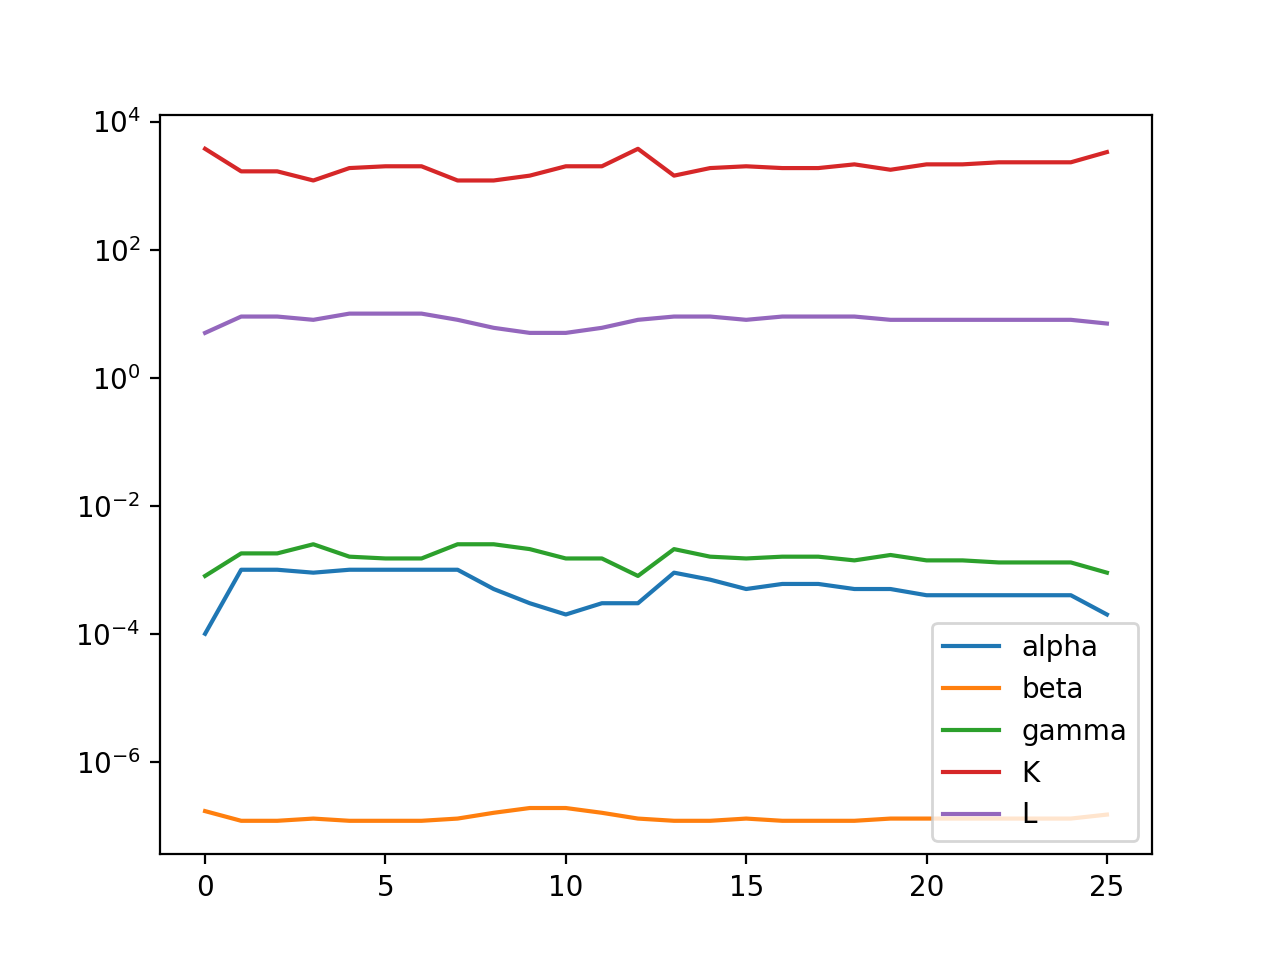
\includegraphics[width=.9\hsize]{bilder/parametrar_over_tid_20200417_evgkf.png}
\caption{Med felfunktion $e_{EVGKF}$}
\end{subfigure}
\caption{Optimala parametrar över tid.}\label{Fig: Parametrar över tid}
\end{figure}
I figur \ref{Fig: Parametrar över tid} är skalan på y-axeln logaritmisk för att vi bättre ska kunna se alla parametrarna i samma figur. Som vi ser förändras inte parametrarna speciellt mycket över tid. Parametrarna ändras nästan inte alls när vi använder $e_{GKF}$, detta beror på att varje dag vi lägger till får en väldigt liten (mindre och mindre över tid) påverkan på felfunktionen. Med $e_{EVGKF}$ ändras parametrarna lite mer, eftersom ny data relativt sett får större inflytande, men även här verkar det som att parametrarna inte påverkas speciellt mycket.

För att belysa hur prediktionen av när toppen ska infalla och dess storlek ändrats över tid plottar vi nu hur tidpunkten för och storleken på toppen har predikterats över tid i följande två figurer:
\begin{figure}[H]
\centering
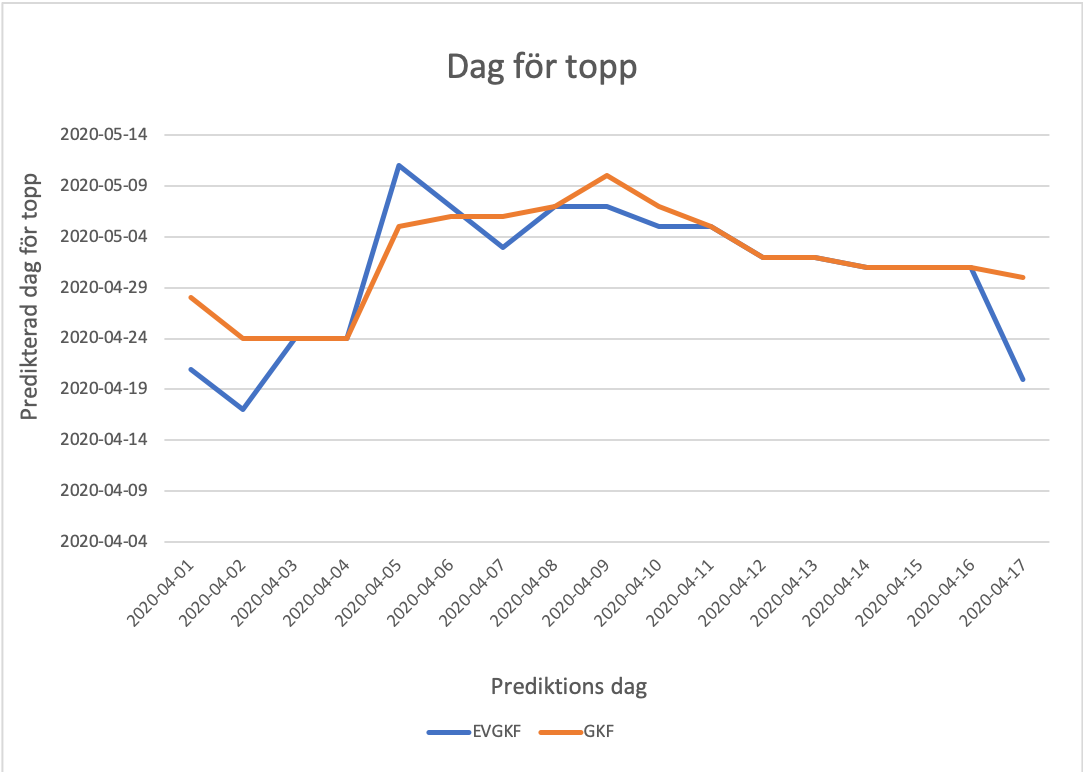
\includegraphics[width=0.6\textwidth]{bilder/predikterad_dag_for_topp_over_tid.png}
\caption{}
\end{figure}
\begin{figure}[H]
\centering
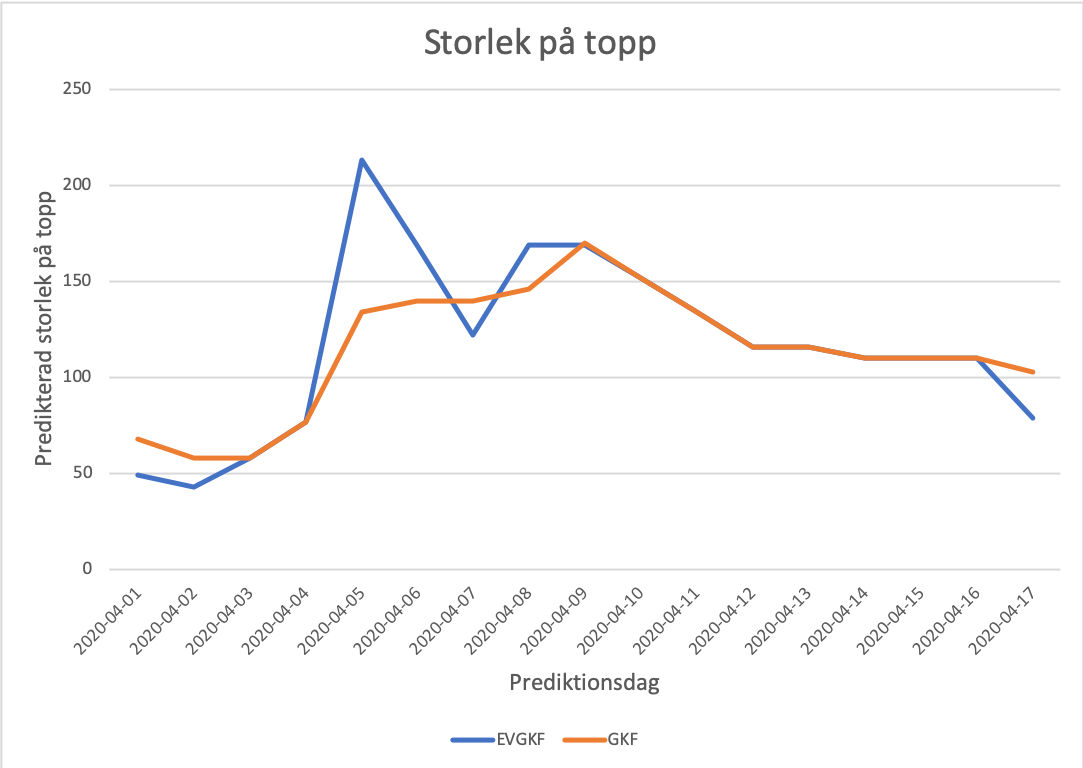
\includegraphics[width=0.6\textwidth]{bilder/predikterad_storlek_pa_topp_over_tid.png}
\caption{}
\end{figure}
Som vi ser i figurerna har prediktionerna för storlek på och tidpunkt för toppen varit väldigt lik med båda felfuktionerna. Dessutom har den varit väldigt lik många dagar i rad. Det innebär att den observerade datan de senaste dagarna varit väldigt nära det som modellen predikterat. Det vi ser då är att toppen den senaste veckan har predikterats att infalla ungefär den 1 maj, och vara på att strax över 100 patienter kommer vara inlagda.

\newpage
\section{Appendix: Utveckling av parametrarnas innebörd}
Vi ska här beskriva varje parameter lite till för att förklara dess innebörd och hur den påverkar förloppet av de olika kategoriernas storlek.

$\alpha$ är andelen som dör när de inte längre har sjukdomen. Denna parameter ändrar bara förhållandet mellan antalet immuna och antalet döda.

$\beta$ är en parameter som i princip säger hur många individer varje sjuk individ smittar. Ett högt $\beta$ innebär att en sjuk individ smittar många från riskgruppen. Detta ger ett snabbare förlopp av hela händelseförloppet samt att det maximala antalet inlagda vid toppen blir högre. Notera att $\beta$ kan bero på individers vanor och rörelsemönster, alltså påverkas denna parameter över tid av exempelvis politiska beslut.

$\gamma$ är andelen av alla individer som är sjuka som blir inlagda. Denna parameter är väldigt svår att skatta och veta vad den borde vara.

$L$ är antalet dagar en individ är sjuk och smittspridare. Större $L$ innebär att varje sjuk individ hinner smitta fler andra.

$K$ är antalet personer som var sjuka den 10 mars. Denna siffra är väldigt svårskattad. Vi kan ha en hyfsad skattning av $K\cdot\gamma$ eftersom vi observerat detta, men förloppet blir väldigt olika beroende på vilken av $K$ och $\gamma$ som är stor.

\end{document}

\iffalse
%% För tre figurer med samma siffra.
\begin{figure}[H]
\centering
\begin{subfigure}[b]{.3\textwidth}
\centering
\includegraphics[width=.99hsize]{AG1RatLinje_HittaM1lsn.png}
\caption{}\label{Fig: AG1RatLinje HittaM1lsn}
\end{subfigure}
\begin{subfigure}[b]{.3\textwidth}
\centering
\includegraphics[width=.9\hsize]{AG1RatLinje_HittaM2lsn.png}
\caption{}
\end{subfigure}
\begin{subfigure}[b]{.3\textwidth}
\centering
\includegraphics[width=.9\hsize]{AG1RatLinje_HittaM3lsn.png}
\caption{}\label{Fig: AG1RatLinje HittaM3lsn}
\end{subfigure}
\caption{}
\end{figure}

%% För två figurer med olika siffror.
\begin{figure}[H]
\centering
\begin{minipage}{.5\textwidth}
\centering
\includegraphics[width=.4\linewidth]{image1}
\captionof{figure}{A figure}
\label{fig:test1}
\end{minipage}
\begin{minipage}{.5\textwidth}
\centering
\includegraphics[width=.4\linewidth]{image1}
\captionof{figure}{Another figure}
\label{fig:test2}
\end{minipage}
\end{figure}

%% För en figur.
\begin{figure}[H]
\centering
\includegraphics[width=0.6\textwidth]{xxx.png}
\caption{}\label{}
\end{figure}

%% För en figur med 3*2 subfigurer
\begin{figure}[t!] % "[t!]" placement specifier just for this example
\begin{subfigure}{0.48\textwidth}
\includegraphics[width=\linewidth]{pic1.pdf}
\caption{First subfigure} \label{fig:a}
\end{subfigure}\hspace*{\fill}
\begin{subfigure}{0.48\textwidth}
\includegraphics[width=\linewidth]{pic2.pdf}
\caption{Second subfigure} \label{fig:b}
\end{subfigure}

\medskip
\begin{subfigure}{0.48\textwidth}
\includegraphics[width=\linewidth]{pic3.pdf}
\caption{Third subfigure} \label{fig:c}
\end{subfigure}\hspace*{\fill}
\begin{subfigure}{0.48\textwidth}
\includegraphics[width=\linewidth]{pic4.pdf}
\caption{Fourth subfigure} \label{fig:d}
\end{subfigure}

\medskip
\begin{subfigure}{0.48\textwidth}
\includegraphics[width=\linewidth]{pic5.pdf}
\caption{Fifth subfigure} \label{fig:e}
\end{subfigure}\hspace*{\fill}
\begin{subfigure}{0.48\textwidth}
\includegraphics[width=\linewidth]{pic6.pdf}
\caption{Sixth subfigure} \label{fig:f}
\end{subfigure}

\caption{My complicated figure} \label{fig:1}
\end{figure}

%%För att göra matriser:
\[
\begin{bmatrix}
    x_{11} & x_{12} & x_{13} & \dots  & x_{1n} \\
    x_{21} & x_{22} & x_{23} & \dots  & x_{2n} \\
    \vdots & \vdots & \vdots & \ddots & \vdots \\
    x_{d1} & x_{d2} & x_{d3} & \dots  & x_{dn}
\end{bmatrix}
\]

%Tabell
\begin{center}
        \begin{tabular}{c|c|c|c}
            Data set & Base 1 & Base 2 & Base 3 \\ \hline
            Training data & 821 & 860 & 945 \\ \hline
            Test data & 795 & 649 & 697 \\ \hline
        \end{tabular}
    \end{center}
\fi
